%%%%%%%%%%%%%%%%%%%%%%%%
%% Cleaning it Up
% get cref working https://tex.stackexchange.com/questions/62611/how-to-make-ref-references-include-the-word-figure
%
%%%%%%%%%%%%%%%%%%%%%%%%
%% After turning it in
% make videos of my results + upload after the report deadline
% clean up code (so it is presentable on Github)
%
%%%%%%%%%%%%%%%%%%%%%%%%

\documentclass[conf]{new-aiaa}
%\documentclass[journal]{new-aiaa} for journal papers
\usepackage[utf8]{inputenc}
\usepackage{amsmath}
\usepackage{color,soul}
\usepackage{gensymb}
\usepackage{graphicx}
\usepackage[version=4]{mhchem}
\usepackage{siunitx}
\usepackage{longtable,tabularx}
\setlength\LTleft{0pt}
\newcommand{\TODO}[1]{\textcolor{red}{\texttt{TODO: }#1}}

\title{Visual Recognition of Lane Markers for Autonomous Road-Going Vehicles}

\author{Jacob Heglund\footnote{Aerospace Engineering, jheglun2@illinois.edu}}
\affil{University of Illinois Urbana-Champaign, Urbana, IL, 61801}

\begin{document}

\maketitle

\begin{abstract}
% The abstract should appear at the beginning of your paper. It should be one paragraph long (not an introduction) and complete in itself (no reference numbers). It should indicate subjects dealt with in the paper and state the objectives of the investigation. Newly observed facts and conclusions of the experiment or argument discussed in the paper must be stated in summary form; readers should not have to read the paper to understand the abstract.
We develop three computer vision-based pipelines for the task of lane detection in autonomous road-going vehicles.  We examine the individual steps necessary to build these pipelines, compare the outputs of the pipelines, and discuss the performance of the pipelines in several real-world scenarios.

\end{abstract}

\section{Introduction}
\label{section: introduction}
% paragraph - define problem, describe its importance, describe SOTA for solving the problem,
The earliest example of autonomous technology in a vehicle sold to the general public was LIDAR-based adaptive cruise control, which was first introduced for consumer vehicles in the mid-1990’s.  Since then there have been many developments including automatic collision avoidance, which is currently on its way to becoming a standard feature in modern cars, and Tesla’s ”Autopilot” feature, which is currently operating in limited highway-driving scenarios. The development of early autonomous road-going technologies was largely the result of investments by automobile manufacturers, but in the modern era autonomous technologies are the result of competition between automobile manufacturers and Silicon Valley-based technology companies.

% paragraph - motivate your work. Why are you writing this paper?
There is clearly a great deal of interest from both industry and academia in developing autonomous technologies. My advisors, Professor Huy Tran and Professor Girish Chowdhary, are both researching the applications of autonomous vehicles, and the topic of autonomy is central to my graduate studies.  However, I have not yet had the opportunity to review and learn about the algorithms that allow autonomous vehicle to navigate visually.  In particular, I have not previously had the opportunity to explore the use of computer vision in the context of autonomous road-going vehicles. Therefore, my goal for this project is the following: develop end-to-end pipelines for detecting lane lines from camera images taken from a road-going vehicle.

% paragraph - talk about initial project goals and issue pinning down the exact work I would do
This project began with the overly ambitious goal of designing an autonomous vehicle that could solve the planning and navigation tasks in a simulated city environment while simultaneously following the laws of the road and safely navigating local obstacles.  This was eventually pared down to solving the high- and low-level navigation tasks separately, but the range of topics was still too broad.  While searching for simulators that would satisfy the initial project goals, I found several simulators developed by Udacity for their "Self Driving Car Engineer Nanodegree" program.  It was the discovery of this program that pushed me to focus on the vision portion of an autonomous vehicle.  The work done for this project is the combination of two projects presented as part of the nanodegree program.

\section{Background}
\label{section: background}
As the number of autonomous vehicles deployed on public roads has increase in recent years, so too has the need for engineers to understand each component of these vehicle systems in order to reduce the risk of accidents caused by system failures.  This section introduces the basic components used to develop lane detection pipeline using only visual information gathered from cameras.  Since we used classical computer vision techniques to process the images, we used the OpenCV Python bindings extensively during this work.  OpenCV is a standard tool in the computer vision research community, and the library is natively written in C++ allowing its use for real-time computer vision tasks.

% subsections - specific CV techniques used for these pipelines + equations
\subsection{Color Thresholding}
RGB is the standard color space for many tasks, but there are also other color spaces that provide unique advantages in detecting certain objects.  The color spaces considered for this report were the RGB, HLS, HSV, LAB, and LUV spaces. As we can see in \ref{fig:color_spaces}, each color space provides a unique perspective on the same image.  By using the channels in which our desired object is brightest, we can easily filter out other objects by setting a threshold for pixel intensity in a particular channel.

This exploration of the color spaces shows that the S-channel of the HLS color space, as well as the R- and G-channels of the RGB color space are very effective at picking out the yellow and white lane markers on the left and right sides of the image respectively.  This allows us to effectively choose channels that will aid in detection of the lane markers.  Note that the example image was taken in bright sunlight on an asphalt road.  Similar explorations would be done for differing lighting conditions, such as nighttime with street lights, or with different colored roads. Also, while a static threshold would work well for static scenes, further work must be done for a camera moving through a scene.

\begin{figure}[h!]
    \centering
    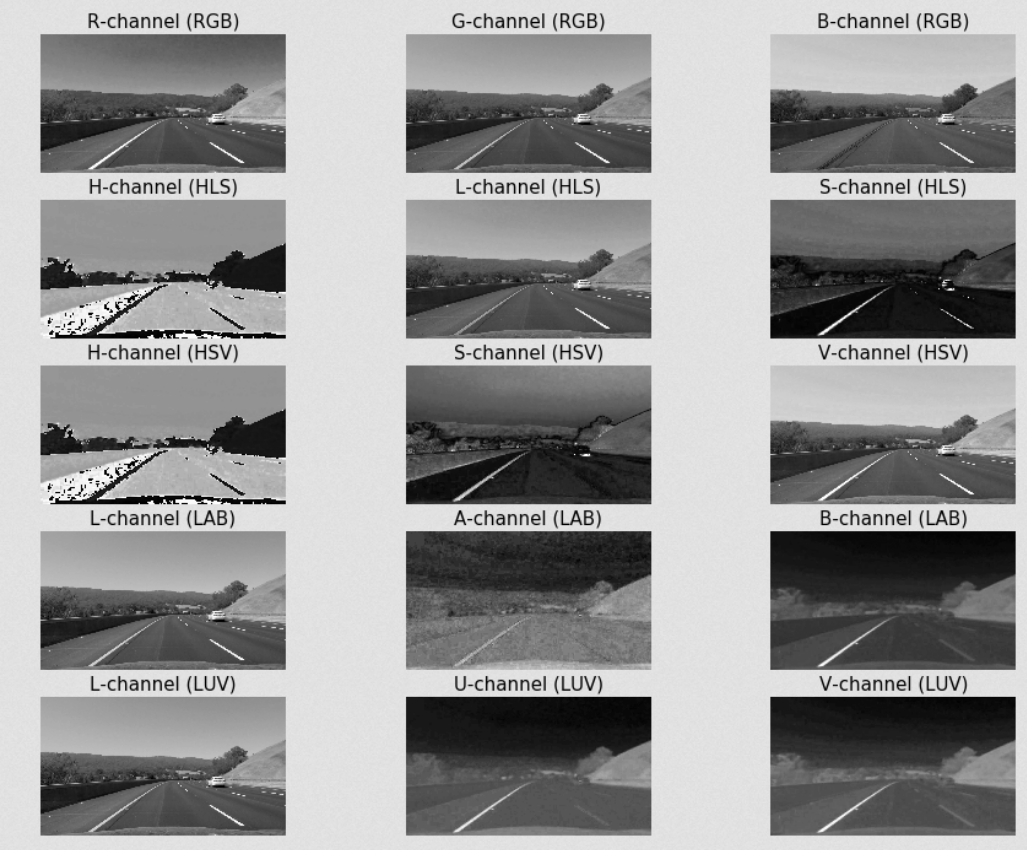
\includegraphics[scale = 0.75]{./images/color_spaces}
    \caption{A comparison of the same image in the different channels of the RGB, HLS, HSV, LAB, and LUV color spaces}
    \label{fig:color_spaces}
\end{figure}

\subsection{Region of Interest Selection}
A region of interest is useful for situations in which the input image contains more information than is required for a particular task.  In the case of lane marker detection in a highway-driving context, we choose our region of interest to be a narrow alley of pixels in the center of the image, as can be seen in \ref{fig:basic_region}.  In this case, the region was manually selected, and would not work well for situations with very wide lanes, such as on a racetrack, or for a steep hill, where more of the lane markers would fall above the region of interest.

\begin{figure}[h!]
    \centering
    \includegraphics[scale = 0.75]{"./images/basic_region"}
    \caption{A typical region of interest for the lane marker detection task}
    \label{fig:basic_region}
\end{figure}

\subsection{Perspective Transformation}
A perspective transformation maps a set of pixels in the original image to a set of pixels in the transformed image.  The transformed image is then easier to analyze with computer vision techniques, as any input perspective can be transformed to a standardized output perspective.  For the lane detection task, we set the new perspective as a "bird's eye" perspective.
We can see this in \ref{fig:adv_perspective2}, where the red circles in the left image are mapped to the red circles in the right image.

This process makes the lane marker detection process easier by transforming intersecting lines to parallel lines in the transformed image.  This transformation implicitly sets a region of interest as well, and requires the designer to choose the pixels that are mapped and the set of pixels they are mapped onto.

\begin{figure}[h!]
    \centering
    \includegraphics[scale = 0.35]{"./images/adv_perspective2"}
    \caption{A demonstration of the original image (left) and the perspective transformed image (right).  The image on the right is used as input for more sophisticated lane marker detection pipelines}
    \label{fig:adv_perspective2}
\end{figure}

\subsection{Canny Edge Detection}
Edges are typically found in regions of high gradient in an image.  The Canny Edge Detection algorithm finds edges within an image by first apply a Sobel operator to calculate the gradient of the image $A$,

\begin{equation}
    G_{x} = \begin{bmatrix}
            -1 & 0 & 1 \\
            -2 & 0 & 2 \\
            -1 & 0 & 1
    \end{bmatrix}
    * A
\end{equation}

\begin{equation}
    G_{y} = \begin{bmatrix}
            -1 & -2 & -1 \\
            0 & 0 & 0 \\
            1 & 2 & 1
    \end{bmatrix}
    * A
\end{equation}
where $G_{x}, G_{y}$ are the gradients in the x and y directions, and $*$ is the convolution operator.  The algorithm then accepts regions with gradient above a certain threshold as edges, and rejects other regions.  As an example, see \ref{fig:cv_canny}.  For the task of detecting lane markers, applying a Canny edge detector is an obvious choice, due to the contrast between the lane markers and the road.  OpenCV also has an implementation available, making the usage of this algorithm simple.
\begin{figure}[h!]
    \centering
    \includegraphics[scale = 0.75]{"./images/cv_canny"}
    \caption{A demonstration of Canny edge detection applied to an image of a road.}
    \label{fig:cv_canny}
\end{figure}

\subsection{Hough Transformation}
The Hough transformation expresses a point $(x,y)$ in terms of $(r, \theta)$, where r is the radius from the origin and $\theta$ is the angle between the radial line and the x-axis.  The algorithm uses this fact to determine if two points lie on the same line by finding intersections in the space parameterized by $(r, \theta)$.  For lane detection, the Hough transformation is most useful if applied after Canny edges have been extracted from an image.  As an output, the Hough transformation gives a set of lines that are most likely to lie along lane markers.

\section{Methodology}
\label{section: methodology}

\subsection{Pipeline 1}
We hypothesized that the color and position of pixels belonging to lane markers were the most important features for effectively detecting lane markers.  In order to test this hypothesis, this pipeline uses a combination of region of interest and color space techniques introduced in Section \ref{section: background}.  We first apply the region of interest mask to the input image.  A threshold on the "red" value of the RGB pixels is then applied so pixels with a red value lower than 175 (on a scale of 0-255) are set to black, and pixels with a red value higher than 175 are set to white.  The value 175 was chosen by testing the threshold filter on several available images.  This creates a binary image with the lane marker pixels highlighted in white, and all other pixels set to black.  By then combining this binary image with the region of interest, we achieve the desired result of individual pixels classified as either lane markers or not lane markers.  Note that this pipeline only considers static images, and does not consider the motion between frames.

\subsection{Pipeline 2}
This pipeline was the first that we developed that applied more-sophisticated computer vision algorithms to the task of lane marker detection.  We first apply a grayscale filter and Gaussian blur to the image for easier processing by the Canny edge detection algorithm.  Then, after extracting the Canny edges (as can be seen in \ref{fig:cv_canny}), we apply OpenCV's implementation of the Hough transformation.  This function returns a set of Hough lines, each parameterized by two coordinates $(x_{1}, y_{1}), (x_{2}, y_{2})$.  We then sort each Hough line into the "left" or "right" lane marker categories for Hough lines with positive and negative slope lines respectively.  Since these Hough lines will not all come from pixels comprising the lane markers, we take the average coordinate from the set of left and right lines $(\overline{x_{1}}, \overline{y_{1}}), (\overline{x_{2}}, \overline{y_{2}})$, and fit a final lane-marker-approximating line to these coordinates. This gives a lane-marker-approximating line for both the left and right lane markers.  By then coloring in the area between these lines and combining with the original image, we not only have a linear approximation of the lane markers, but also have a rudimentary method for differentiating the lane in front of the vehicle from the rest of the road.

So far, we have only considered still images, but the line fitting done in this pipeline allowed us to track the fit coefficients over time.  Since the dataset we used comprised of highway driving scenarios, we made the assumption that the fit coefficients will not change quickly due to rapidly changing road conditions.  Therefore, we took the average fit coefficients of the current frame with the past ten frames, and set this as our current fit.  This addition to the pipeline smooths the response of the lane detector and makes it less susceptible to noise caused by deviations in the road surface.


\subsection{Pipeline 3}
We combined computer vision techniques and sophisticated lane marker tracking to develop this pipeline.  We first apply a perspective transformation \ref{fig:adv_perspective2} so the image of the road in front of the vehicle is easier to process.  We then apply color space filtering and Canny edge detection to get a binary image of the pixels belonging to the lane markers.  By applying a histogram along the x-axis of the binary image, we find two peaks that correspond to the left and right lane markers.  We then create a window of interest around each peak near the bottom of the image.  The width of the windows is chosen with the knowledge that lane markers are relatively narrow objects, and the height of the window is chosen such that it divides the height of the image with no remainder.

After the pixels in the first window are stored in memory, the window slides up a prescribed amount and identifies further pixels belonging to the lane markers.  The sliding window of interest method is effective because it only identifies pixels that are close to the lane markers, and therefore provides a more robust method for detecting the lane markers.  The result of this process can be seen in \ref{fig:adv_sliding_window}.  We fit a 2nd order polynomial to the pixel positions, color in the space between the curves, and invert the perspective transformation to get the final result.  This method is the most sophisticated implemented for this project, and allows us to also calculate the radius of curvature \ref{eqn:radius of curvature} through visual sensing alone, as well as the vehicle's position within the lane.

\begin{equation}
    \label{eqn:radius of curvature}
    R = \dfrac{(1+\dfrac{dy}{dx}^2)^{\dfrac{3}{2}}}{\dfrac{d^2 y}{dx^2}}
\end{equation}

We also incorporated curve fit smoothing between frames of the input video by storing the previous fit coefficients in memory, and calculating the new lane marker fit as a moving average.

\begin{figure}[h!]
    \centering
    \includegraphics[scale = 0.65]{"./images/adv_sliding_window"}
    \caption{The result of the sliding window of interest method for identifying lane markers}
    \label{fig:adv_sliding_window}
\end{figure}

\section{Results and Discussion}
\label{section: results}
Since still images on a report do not effectively convey the action of the lane detectors, videos and source code for these lane detectors can be found at \textbf{https://github.com/jacob-heglund/self-driving-car}.

% paragraph - results of pipeline 1 + images
\subsection{Pipeline 1}
The output of this pipeline is a set of pixels that are identified as being part of the lane markers, and can be seen in \ref{fig:basic_shaded}. While the pipeline is not sophisticated, it did lay the groundwork for the use of color space and region of interest techniques in the later pipelines.  Also, it was not immediately obvious that exploring the different color spaces would be useful for this task, so it was surprising that such a simple technique could prove effective.

% paragraph - assumptions and where they would break
One of the core assumptions that this detector makes is that the color of the lane markers in the United States must be either yellow or white.  This color scheme is mandated by federal law for regular roads, however bike lanes with green markings or construction zones with orange markers would contradict the current assumptions, and the detector must be adjusted to handle these cases as well.  The detector also assumes that the lane markers are the only type of white and yellow markings on the road.  However in a city scenario, lane markers would look very similar to pedestrian crossing markers, and the detector would not be able to operate effectively in that situation.

\begin{figure}[h!]
    \centering
    \includegraphics[scale = 0.5]{"./images/basic_final"}
    \caption{The result of the first computer vision pipeline}
    \label{fig:basic_shaded}
\end{figure}

\subsection{Pipeline 2}
% paragraph - results of pipeline 2 + images
The idea behind this lane detector was to incorporate more generalizable techniques from classical computer vision.  By using Canny edge detection in conjunction with the Hough transformation, we have a pipeline with relatively few tunable parameters that gives an approximate fit for the lane markers.  This lane detector also yields a region of the image that approximates the lane in front of the vehicle, which could be used as part of a hazard detection pipeline that runs in parallel with the lane marker detection pipeline.

% paragraph - assumptions and where they would break
Similar to the first detector, this detector assumes that lane markers are the primary markings on the road surface.  For highway driving, this assumption holds, but cities would provide a greater challenge to a lane marker detector.  The accuracy of the lane marker fit would be decreased, since there is currently no filtering of horizontal or nearly horizontal lines in the image.  In addition, rapid changes in lighting conditions, such as shadows on the road surface, would pose a problem to the Canny edge detection and Hough transformation algorithms.  For small regions covered by shadows, some form of smoothing that rejects quick changes in line fit would be effective, but for a road running through a forest, the constantly changing lighting conditions would pose a serious challenge.

\begin{figure}[h!]
    \centering
    \includegraphics[scale = 0.5]{"./images/cv_final"}
    \caption{The result of the second computer vision pipeline}
    \label{fig:cv_final}
\end{figure}

\subsection{Pipeline 3}
% paragraph - results of pipeline 3 + images
This pipeline extends the notion of a region of interest with the perspective transformation and the sliding window of interest.  While the perspective transformation still relies on a manually chosen set of points, there are potentially fewer parameters with the perspective transformation and the output is more useful for analysis further down the pipeline.  Similarly, the sliding window of interest method provides a more robust detector for lane marker pixels while reducing the number of parameters.  As an output, this pipeline also detects the lane in front of the vehicle,like the second pipeline.  This allows other features of interest, such as obstacles, to be easier detected.

% paragraph - assumptions and where they would break
This detector shares has many of the same weaknesses as the other detectors.  Along with sensitivity to rapidly changing lighting conditions and other markings on the road, this detector also requires the two lane markers to be in sight to generate an estimated fit.  In an intersection where the lane markers are briefly not available, this would pose a challenge, especially for a turning vehicle.  One potential solution is to incorporate vehicle motion models and motion prediction into the lane detector algorithm, which would limit the detector's influence on other parts of the autonomous system in situations where lane markers are not available.

\begin{figure}[h!]
    \centering
    \includegraphics[scale = 0.65]{"./images/advanced_final"}
    \caption{The result of the third computer vision pipeline}
    \label{fig:advanced_final}
\end{figure}

% subsection - moving forward
% paragraph - CV vs deep learning
% CV - easy for first iterations, but difficult to generalize
\subsection{Computer Vision and Deep Learning}
Classical computer vision pipelines often rely on an explicit model of a domain combined with a carefully chosen set of heuristics.  The pipelines developed for this project were developed for the sole purpose of lane-marker detection.  If we wanted to extend our pipeline to also detect other obstacles, it would almost certainly require a complete re-working of the pipeline.  Certain assumptions we made about the location of the object in the scene would break, color-based techniques may not be effective, the Hough transformation would not pick out useful features, and Canny edges may not have a meaningful interpretation.  As it stands, classical computer vision techniques can be very useful, as long as the scope is well-defined.

% DL -it's ability to generalize, but requires data
If we want a model that is able to generalize to multiple tasks, deep learning seems to provide a solution.  Deep learning has become a topic of interest in the area of computer vision, mainly due to the ability of deep learning models to generalize in difficult tasks.  The promise of deep learning is that more data yields higher model accuracy, and this has mostly proven true in many other contexts.  For autonomous road-going vehicles, the task of detecting lane markers and other objects in the scene can be solved with a single deep learning model.  However, deep learning models can act unpredictably and uncertainty quantification is still an area of active research.  For this reason, end-to-end solutions are typically not desirable in safety-critical applications, and a more sophisticated object-detection system would incorporate deep learning with classical computer vision techniques to allow more predictable behavior.

\section{Conclusion}
\label{section: conclusion}
% A conclusion section is not required, though it is preferred. Although a conclusion may review the main points of the paper, do not replicate the abstract as the conclusion. A conclusion might elaborate on the importance of the work or suggest applications and extensions. \textit{Note that the conclusion section is the last section of the paper that should be numbered. The appendix (if present), acknowledgment, and references should be listed without numbers.}

% paragraph - takeaways
Overall this project was a great success on the dimensions of learning and presentable results.  Before starting this project, I had only basic knowledge of image processing with computer vision techniques, and had never written the pipelines from scratch.  This process of learning and implementing has had the effect that I would now feel comfortable in tackling computer vision tasks in other domains as well. Computer vision is vital to the operation of autonomous vehicles in nearly every domain, and I am now more well-rounded as a researcher in the area of autonomy. In terms of presentable results, the lane detectors have been shown to be effective in their design domains, and if this work were part of the development of a real autonomous vehicle, this work would form a foundation on which more sophisticated visual systems could be built.

I would like to thank Professor Grace Gao for her helpful feedback in formulating my original project topic, as well as helping me to focus on a specific aspect of autonomous vehicles.  I would also like to thank my fellow AE 598 Advanced Navigation Systems students for their feedback during my midterm and final project presentations.


\section*{References}
\begin{enumerate}
    \item Udacity, 2019.  CarND-LaneLines-P1.

    https://github.com/udacity/CarND-LaneLines-P1


    \item Udacity, 2019.  CarND-Functional-Safety-Project

    https://github.com/udacity/CarND-Functional-Safety-Project

    \item Udacity, 2019.  CarND-Advanced-Lane-Lines.

    https://github.com/udacity/CarND-Advanced-Lane-Lines


    \item PyData, 2017, July 26.  Ross Kippenbrock - Finding Lane Lines for Self Driving Cars.

    https://www.youtube.com/watch?v=VyLihutdsPk

  \end{enumerate}

\end{document}




















